\documentclass[aspectratio=169]{beamer}
 
\usetheme[sectionpage=none, subsectionpage=none, progressbar=none]{metropolis}           % Use metropolis theme
 
  \usepackage{outlines}
  \usepackage{caption}
  \usepackage{appendixnumberbeamer}
  \usepackage{booktabs}
  \usepackage{tcolorbox}
  \usepackage{tabularx}
  \usepackage[export]{adjustbox}[2011/08/13]
  \usepackage{bm}

\newcolumntype{R}{>{\raggedleft\arraybackslash}X} 
  
 \setbeamertemplate{footline}[frame number]{}

\setbeamertemplate{footline}{% 
  \hfill% 
  \usebeamercolor[fg]{page number in head/foot}% 
  \usebeamerfont{page number in head/foot}% 
  \insertframenumber%
  %\,/\,\inserttotalframenumber
  \kern1em\vskip2pt% 
}

\makeatletter
\setbeamertemplate{headline}{%
  \begin{beamercolorbox}[colsep=1.5pt]{upper separation line head}
  \end{beamercolorbox}
  \begin{beamercolorbox}{section in head/foot}
    \vskip2pt\insertnavigation{\paperwidth}\vskip2pt
  \end{beamercolorbox}%
  \begin{beamercolorbox}[colsep=1.5pt]{lower separation line head}
  \end{beamercolorbox}
}
\let\@@magyar@captionfix\relax % IMPORTANT: This is a workaround to fix a random eror with the 2018 installation
\makeatother

\usepackage{xcolor} 
\listfiles

\setbeamercolor{section in head/foot}{fg=normal text.bg, bg=structure.fg}

    \usepackage{smartdiagram}
    \usepackage{tikz}
\usetikzlibrary{shapes.geometric, arrows}
\tikzstyle{startstop} = [rectangle, rounded corners, minimum width=3cm, minimum height=1cm,text centered, draw=black, fill=red!30]
\tikzstyle{io} = [trapezium, trapezium left angle=70, trapezium right angle=110, minimum width=3cm, minimum height=1cm, text centered, draw=black, fill=blue!30]
\tikzstyle{process} = [rectangle, minimum width=3cm, minimum height=1cm, text centered, draw=black, fill=orange!30]
\tikzstyle{decision} = [diamond, minimum width=3cm, minimum height=1cm, text centered, draw=black, fill=green!30]

\title{Gov 2006: Formal Political Theory II \\
Section 4}
\date{\today}
\author{ \textbf{Sophie Hill}}


\begin{document}
  \maketitle
  

%%%%%%%%%%%%%%%%%%%%%%%%%%%%%%%%%%%%%%%%%%
\begin{frame}{Agenda}

\Large

\begin{itemize}
\setlength{\itemsep}{1.5em}

\item PSET review: (even more) probabilistic voting 

\item Models of growth \& inequality 

\item Brainstorming: what's missing?

\end{itemize}

\end{frame}
%%%%%%%%%%%%%%%%%%%%%%%%%%%%%%%%%%%%%%%%%%
\begin{frame}{PSET review}

We start with the familiar set-up:

\begin{itemize}
\item $W(q^P, \alpha^i)$ = indirect utility for voter $i$ from policy $q^P$
\item individual shock $\sigma_i \sim U \left[ -\frac{1}{2 \phi}, \frac{1}{2 \phi} \right]$  
\item aggregate shock $\delta \sim U \left[ -\frac{1}{2 \psi}, \frac{1}{2 \psi} \right]$ 

\pause 
\vspace{2em}
\noindent Now define $\tilde{\sigma}^i$ as the value that makes voter $i$ indifferent between $A$ and $B$:


$$ \tilde{\sigma}^i(\alpha^i, q^A, q^B, \delta) = W(q^A, \alpha^i) - W(q^B, \alpha^i) - \delta $$


\end{itemize}
\end{frame}
%%%%%%%%%%%%%%%%%%%%%%%%%%%%%%%%%%%%%%%%%%
\begin{frame}{PSET review}

For each voter $i$, the probability that they vote for $A$ depends on their realization of $\sigma^i$:

\pause
\begin{eqnarray*}
p_i^A &=& Prob \left[ \sigma^i \leq \tilde{\sigma}(\alpha^i, q^A, q^B, \delta) \right] \\
\pause 
&=&  \int_{-\frac{1}{2\phi}}^{\tilde{\sigma}(\alpha^i, q^A, q^B, \delta)} \phi \, \, d \sigma^i  \\
\pause
&=& \phi \left[ \tilde{\sigma}(\alpha^i, q^A, q^B, \delta) + \frac{1}{2 \phi} \right] \\
\pause
&=& \phi \left[ W(q^A, \alpha^i) - W(q^B, \alpha^i) - \delta + \frac{1}{2 \phi} \right]
\end{eqnarray*}



\end{frame}
%%%%%%%%%%%%%%%%%%%%%%%%%%%%%%%%%%%%%%%%%%
\begin{frame}{PSET review}

So we can express $\pi^A$, the vote share of $A$, as follows:

\begin{eqnarray*}
\pi^A &=& \int_{\alpha^i} Prob \left[ \sigma \leq \tilde{\sigma}(\alpha^i, q^A, q^B, \delta) \right] dF(\alpha^i) \\
\pause
&=& \int_{\alpha^i} \phi \left[ W(q^A, \alpha^i) - W(q^B, \alpha^i) - \delta + \frac{1}{2 \phi} \right] dF(\alpha^i) \\
\pause
&=& \phi \left[ W(q^A, \alpha) - W(q^B, \alpha) - \delta \right] + \frac{1}{2}
\end{eqnarray*}


\end{frame}
%%%%%%%%%%%%%%%%%%%%%%%%%%%%%%%%%%%%%%%%%%
\begin{frame}{PSET review}

Now -- finally! -- we can write down $p^A$, $A$'s probability of winning:

\vspace{-1em}
\begin{eqnarray*}
p^A &=& Prob \left[ \pi^A > \frac{1}{2} \right]  \\
\pause
&=& Prob \left[ \phi \left( W(q^A, \alpha) - W(q^B, \alpha) - \delta \right) + \frac{1}{2} > \frac{1}{2} \right] \\
\pause
&=& Prob \left[ \phi \left( W(q^A, \alpha) - W(q^B, \alpha) - \delta \right) >0 \right] \\
\pause
&=& Prob \left[ \delta \leq W(q^A, \alpha) - W(q^B, \alpha) \right] \\
\pause
&=& \int_{-\frac{1}{2\psi}}^{W(q^A, \alpha) - W(q^B, \alpha)} \psi d \delta \\
\pause
&=& \psi \left[ W(q^A, \alpha) - W(q^B, \alpha) \right] + \frac{1}{2}
\end{eqnarray*}

\end{frame}

%%%%%%%%%%%%%%%%%%%%%%%%%%%%%%%%%%%%%%%%%%
\begin{frame}{Models of inequality \& growth}

Last week we covered two very influential papers arguing that:

\begin{tcolorbox}
$\uparrow$ inequality \, \,  $\rightarrow$  \, \,  $\uparrow$ redistribution  \, \,  $\rightarrow$  \, \,  $\downarrow$ growth
\end{tcolorbox}

\pause 

\begin{outline}
\1 Alesina \& Rodrik (1994) 
\2 conflict between capital and labor
\2 taxes redistribute but ALSO finances a public good necessary for private production

\1 Persson \& Tabellini (1994) 
\2 overlapping generations model where agents can invest in human capital
\2 taxes are purely redistributive
\end{outline}


\end{frame}
%%%%%%%%%%%%%%%%%%%%%%%%%%%%%%%%%%%%%%%%%%

\begin{frame}{Empirical testing}

\begin{outline}
\1 \textbf{Cross-sectional OLS}: Alesina \& Rodrik (1994), Persson 
\& Tabellini (1994)
\2 inequality \textcolor{red}{decreases} growth

\vspace{2em} 

\invisible<1>{
\1 \textbf{Panel data with country fixed efffects}: Li 
\& Zou (1998), Forbes (2000)
\2 inequality \textcolor{green}{increases} growth

\vspace{2em} 


\1 \textbf{Non-linear specifications}: Banerjee \& Duflo (2003)
\2 \textcolor{blue}{changes} in inequality (in \textit{either direction}) \textcolor{red}{decrease} growth }

\end{outline}

\end{frame}
%%%%%%%%%%%%%%%%%%%%%%%%%%%%%%%%%%%%%%%%%%
\begin{frame}{Empirical testing: cross-sectional OLS}

\begin{figure}
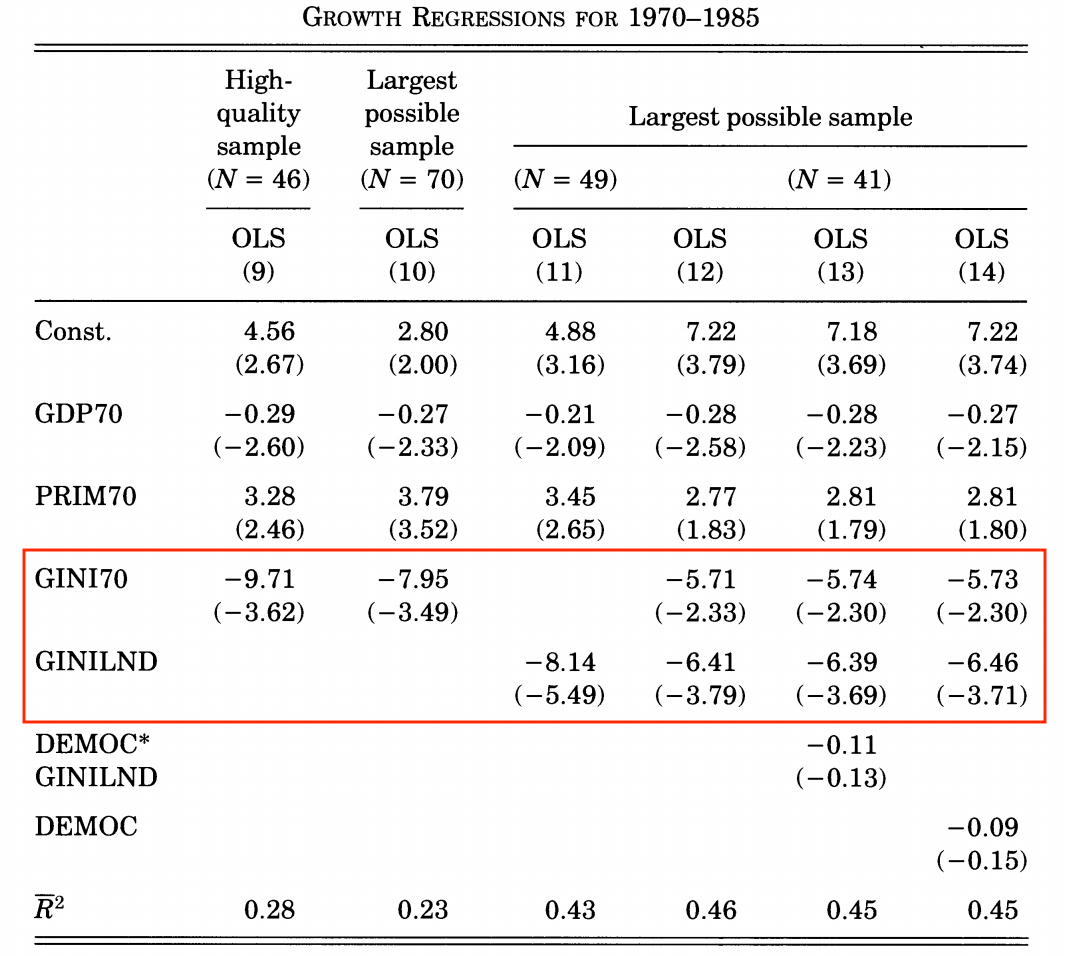
\includegraphics[width=0.5\textwidth]{alesina_tab.png}
\caption*{\footnotesize{Table II from Alesina \& Rodrik, 1994} }
\end{figure}

\end{frame} 

%%%%%%%%%%%%%%%%%%%%%%%%%%%%%%%%%%%%%%%%%%
\begin{frame}{Empirical testing}

\begin{outline}
\1 \textbf{Cross-sectional OLS}: Alesina \& Rodrik (1994), Persson 
\& Tabellini (1994)
\2 inequality \textcolor{red}{decreases} growth

\vspace{2em} 

\1 \textbf{Panel data with country fixed efffects}: Li 
\& Zou (1998), Forbes (2000)
\2 inequality \textcolor{green}{increases} growth

\vspace{2em} 

\invisible<1>{
\1 \textbf{Non-linear specifications}: Banerjee \& Duflo (2003)
\2 \textcolor{blue}{changes} in inequality (in \textit{either direction}) \textcolor{red}{decrease} growth }

\end{outline}

\end{frame}
%%%%%%%%%%%%%%%%%%%%%%%%%%%%%%%%%%%%%%%%%%
\begin{frame}{Empirical testing: panel data with fixed effects}

\begin{figure}
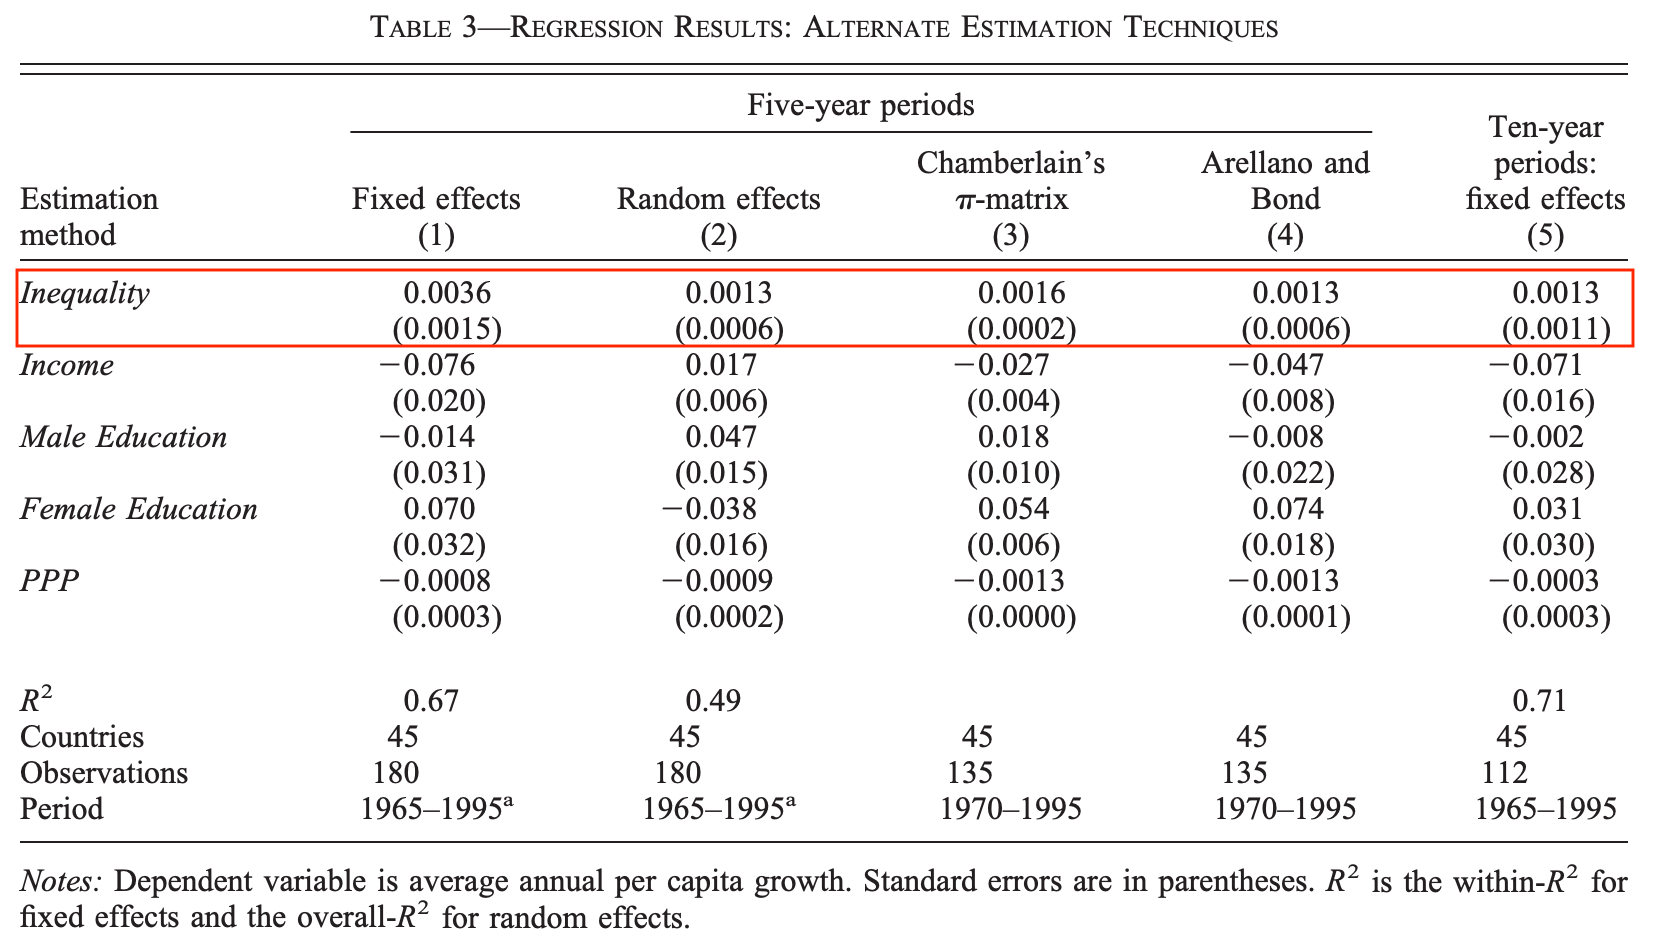
\includegraphics[width=0.8\textwidth]{forbes.png}
\caption*{\footnotesize{Table 3 from Forbes, 2000} }
\end{figure}

\end{frame} 
%%%%%%%%%%%%%%%%%%%%%%%%%%%%%%%%%%%%%%%%%%
\begin{frame}{Empirical testing}

\begin{outline}
\1 \textbf{Cross-sectional OLS}: Alesina \& Rodrik (1994), Persson 
\& Tabellini (1994)
\2 inequality \textcolor{red}{decreases} growth

\vspace{2em} 

\1 \textbf{Panel data with country fixed efffects}: Li 
\& Zou (1998), Forbes (2000)
\2 inequality \textcolor{green}{increases} growth

\vspace{2em} 


\1 \textbf{Non-linear specifications}: Banerjee \& Duflo (2003)
\2 \textcolor{blue}{changes} in inequality (in \textit{either direction}) \textcolor{red}{decrease} growth 

\end{outline}

\end{frame}
%%%%%%%%%%%%%%%%%%%%%%%%%%%%%%%%%%%%%%%%%%
\begin{frame}{Empirical testing: non-linear specification}

\begin{figure}
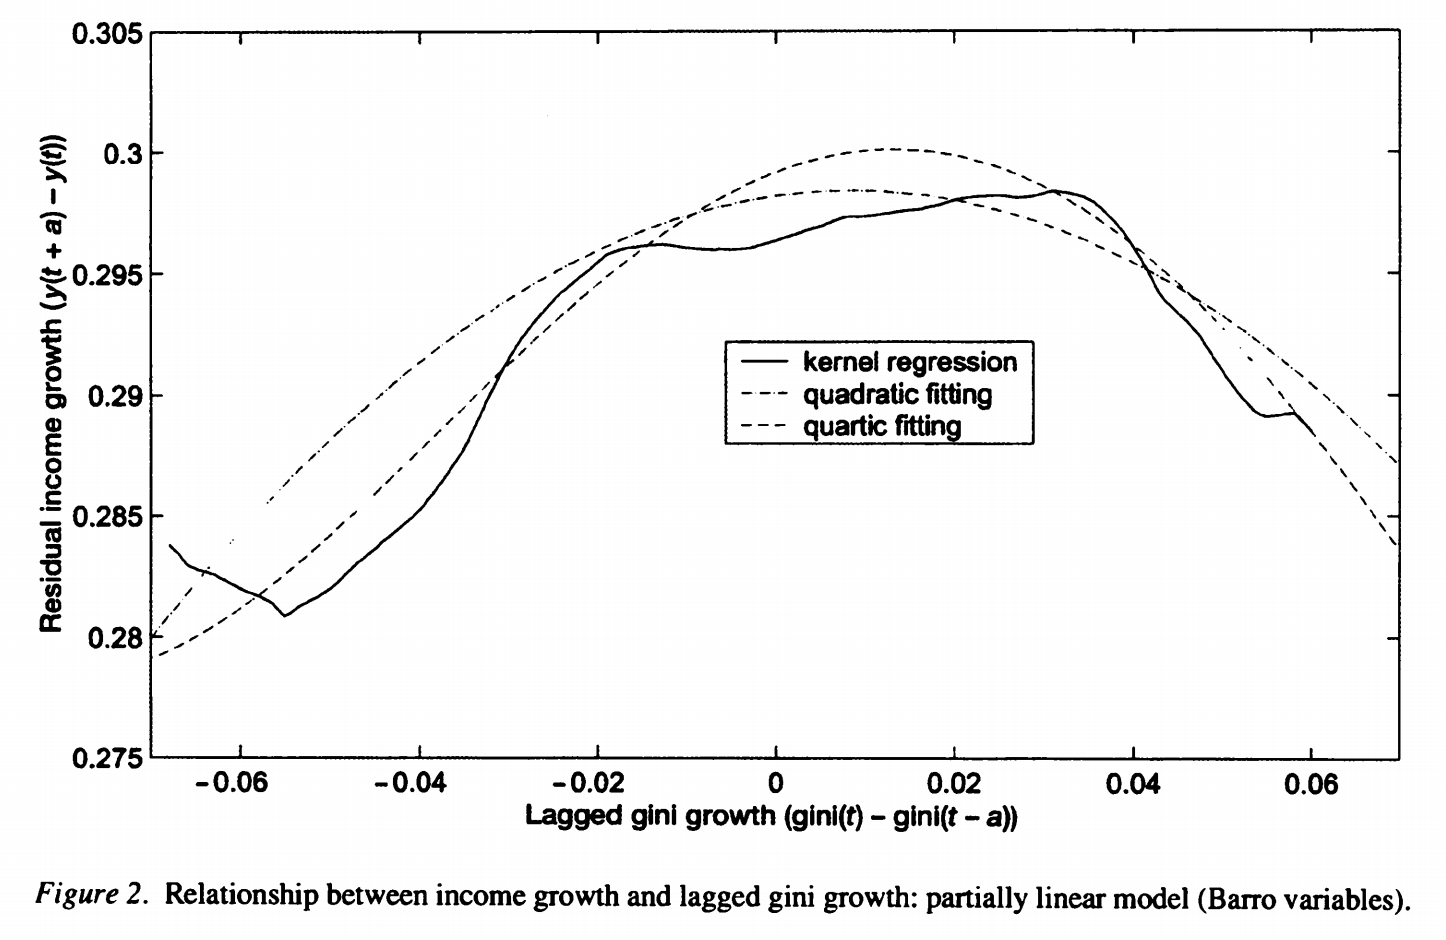
\includegraphics[width=0.65\textwidth]{banerjee.png}
\caption*{\footnotesize{Figure 2 from Banerjee \& Duflo, 2003} }
\end{figure}

\end{frame} 
%%%%%%%%%%%%%%%%%%%%%%%%%%%%%%%%%%%%%%%%%%
\begin{frame}{Empirical testing: what should the data look like?}

\begin{outline}

\1 \textbf{Scope conditions}
\2 Should we expect models based on MVT to apply to all democracies? \pause 
\2 How about real-world \textit{dictatorships}? \pause (A\&R 1994 say yes, P\&T 1994 say no!)

\pause 
\vspace{2em}


\1 \textbf{Periodization}
\2 Long-term growth (e.g. 25 yr period) used in x-sectional OLS
\2 Medium-term growth (e.g. 5 yr periods) used with panel data

\pause 
\vspace{2em}

\pause 
\1 \textbf{Measuring inequality}
\2 Gini coefficient most common, but not a good measure of mean-median skew!
\2 Persson \& Tabellini (1994) is a notable exception, using the income share going to the middle quintile. Better approximation of the position of the median voter?

\end{outline}

\end{frame}
%%%%%%%%%%%%%%%%%%%%%%%%%%%%%%%%%%%%%%%%%%
\begin{frame}{Empirical testing: evidence on the mechanism}

\large 
\begin{itemize}
\item Recall that both Alesina \& Rodrik (1994), Persson 
\& Tabellini (1994) identify (the threat of) \alert{redistribution} as the key mechanism linking inequality and growth. 
\item So far we've only seen evidence on the inequality-growth relationship.
\item Does inequality $\uparrow$ redistribution? And does redistribution $\downarrow$ growth?
\end{itemize}

\end{frame}
%%%%%%%%%%%%%%%%%%%%%%%%%%%%%%%%%%%%%%%%%%
\begin{frame}{Empirical testing: does inequality $\uparrow$ redistribution?}

\begin{figure}
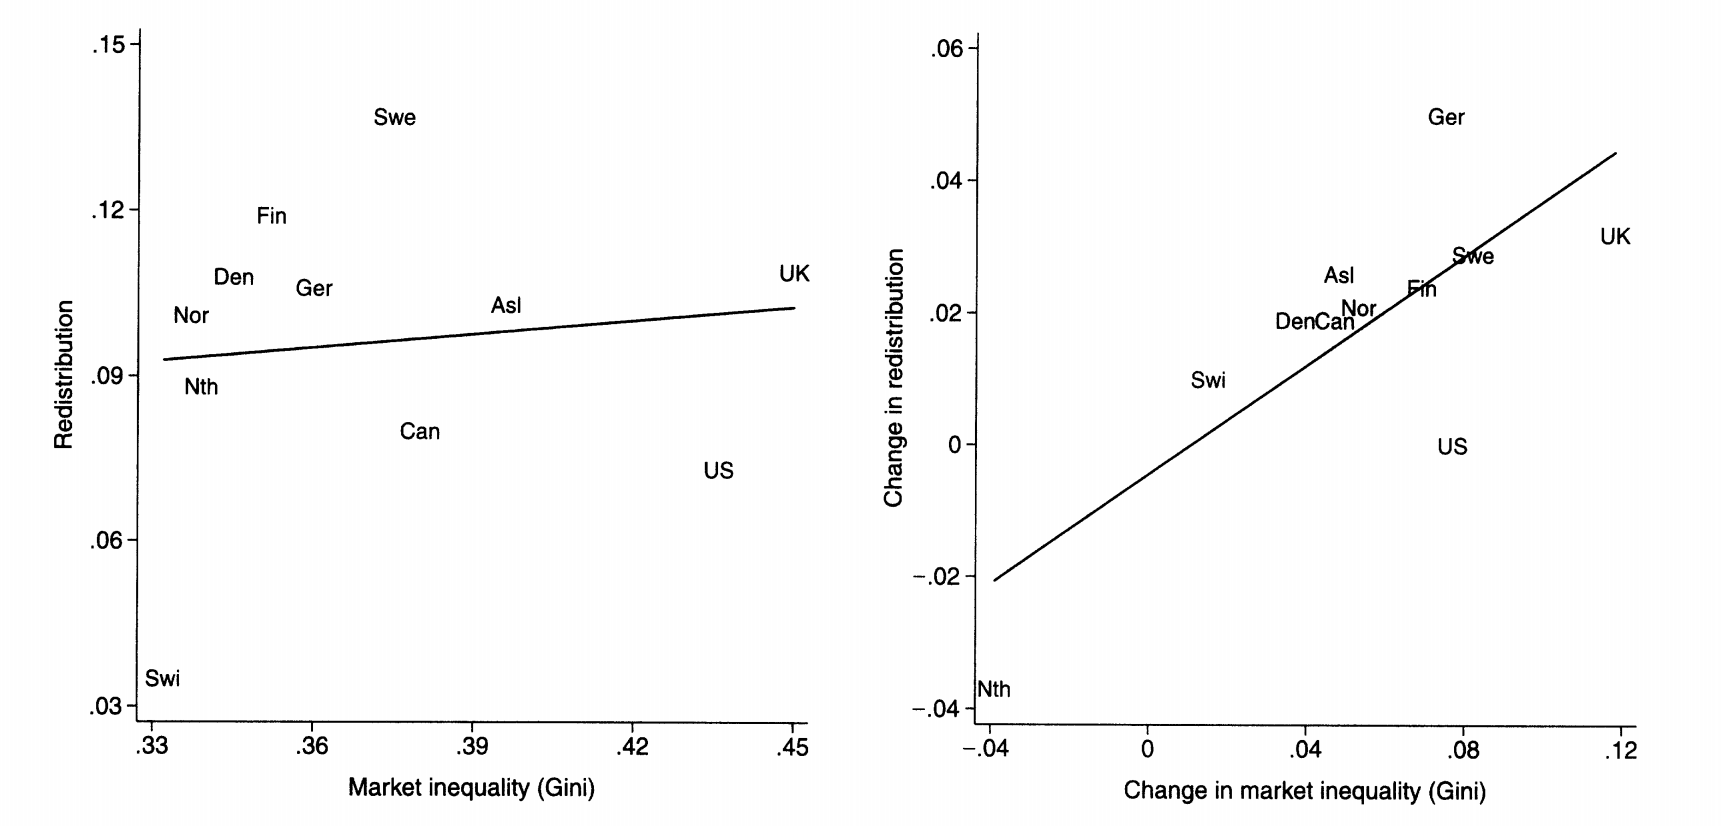
\includegraphics[width=0.9\textwidth]{kenworthy.png}
\caption*{\footnotesize{Figures 6 \& 7 from Kenworthy \& Pontusson, 2005} }
\end{figure}


\end{frame}
%%%%%%%%%%%%%%%%%%%%%%%%%%%%%%%%%%%%%%%%%%

\begin{frame}{Empirical testing: does redistribution $\downarrow$ growth?}

\begin{figure}
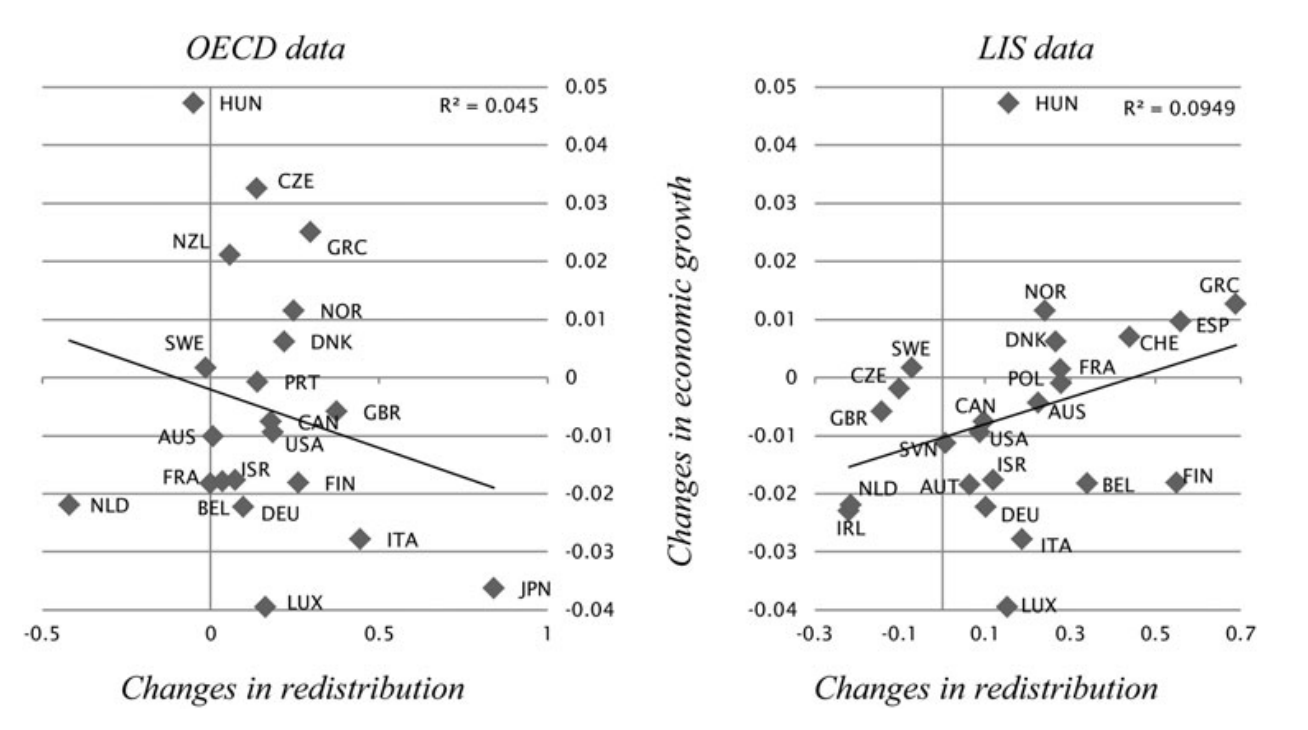
\includegraphics[width=0.9\textwidth]{Thewissen.png}
\caption*{\footnotesize{Figure 7 from Thewissen, 2014} }
\end{figure}


\end{frame}
%%%%%%%%%%%%%%%%%%%%%%%%%%%%%%%%%%%%%%%%%%
\begin{frame}{Let's brainstorm! Round I}

\Large 
What's missing from the A\&R / P\&T models?

\pause 

\vspace{3em}

\begin{tcolorbox}
Drawing on your substantive knowledge, come up with \alert{3 factors} that might complicate the \alert{inequality-redistribution} link or the \alert{redistribution-growth} link.
\end{tcolorbox}
\end{frame}


%%%%%%%%%%%%%%%%%%%%%%%%%%%%%%%%%%%%%%%%%%
\begin{frame}{Let's brainstorm! Round II}

\Large
How can we incorporate these insights into a formal model?

\vspace{3em}


\begin{tcolorbox}
Pick \alert{1 suggestion} and brainstorm how it could be introduced in a formal model, drawing on material we have covered so far.
\end{tcolorbox}


\end{frame}
%%%%%%%%%%%%%%%%%%%%%%%%%%%%%%%%%%%%%%%%%%
\begin{frame}{Section feedback}

\Large

As always, your feedback on how to improve section is much appreciated!

\vspace{2em}

Feedback form: \url{https://goo.gl/forms/qYk5zoI4yOShpDxo2}


\end{frame}


\end{document}